\documentclass[a4paper,12pt]{article} % The document class with options

\usepackage[T1]{fontenc}
\usepackage{enumitem}
\usepackage{amsmath}
\usepackage{amsfonts}
\usepackage{microtype}
\usepackage{graphicx}
\usepackage{epstopdf}
% \usepackage{float}
% chktex-file 1
% chktex-file 3
% chktex-file 15
% chktex-file 18

\begin{document}
\setlength{\parskip}{1em} 
\setlength{\parindent}{0pt}
\newcommand{\vect}[1]{\mathbf{#1}}
\title{MECH 503 Homework 2}
\author{Jincong Li \\ 60539939}
\date{Feb 16th}
\maketitle

\section*{Q1}
\begin{align*}
    \vect{u} &= \left[\begin{matrix}x_{1}^{3} + x_{1} x_{2}^{2} + x_{3}^{2}\\- x_{2}^{3} + x_{3}^{2}\\- x_{1}^{3} + 2 x_{1} x_{2} x_{3}\end{matrix}\right] \\
    \nabla \vect{u}  &= \left[\begin{matrix}3 x_{1}^{2} + x_{2}^{2} & 2 x_{1} x_{2} & 2 x_{3}\\0 & - 3 x_{2}^{2} & 2 x_{3}\\- 3 x_{1}^{2} + 2 x_{2} x_{3} & 2 x_{1} x_{3} & 2 x_{1} x_{2}\end{matrix}\right] \\
    {\nabla \vect{u}}^{T} &= \left[\begin{matrix}3 x_{1}^{2} + x_{2}^{2} & 0 & - 3 x_{1}^{2} + 2 x_{2} x_{3}\\2 x_{1} x_{2} & - 3 x_{2}^{2} & 2 x_{1} x_{3}\\2 x_{3} & 2 x_{3} & 2 x_{1} x_{2}\end{matrix}\right] \\
    \intertext{Thus, the infinitisimal strain tensor is determined to be:}
    \vect{\varepsilon} &= \left[\begin{matrix}3.0 x_{1}^{2} + 1.0 x_{2}^{2} & 1.0 x_{1} x_{2} & - 1.5 x_{1}^{2} + 1.0 x_{2} x_{3} + 1.0 x_{3}\\1.0 x_{1} x_{2} & - 3.0 x_{2}^{2} & 1.0 x_{1} x_{3} + 1.0 x_{3}\\- 1.5 x_{1}^{2} + 1.0 x_{2} x_{3} + 1.0 x_{3} & 1.0 x_{1} x_{3} + 1.0 x_{3} & 2.0 x_{1} x_{2}\end{matrix}\right]
    \intertext{at point $\vect{x}=[1,0,1]^T$,}
    \vect{\varepsilon} &= \left[\begin{matrix}3.0 & 0 & -0.5\\0 & 0 & 2.0\\-0.5 & 2.0 & 0\end{matrix}\right]
    \intertext{The vorticity tensor is}
    \vect{\omega} &= \left[\begin{matrix}0 & 1.0 x_{1} x_{2} & 1.5 x_{1}^{2} - 1.0 x_{2} x_{3} + 1.0 x_{3}\\- 1.0 x_{1} x_{2} & 0 & - 1.0 x_{1} x_{3} + 1.0 x_{3}\\- 1.5 x_{1}^{2} + 1.0 x_{2} x_{3} - 1.0 x_{3} & 1.0 x_{1} x_{3} - 1.0 x_{3} & 0\end{matrix}\right]\\
    \intertext{at point $\vect{x}=[1,0,1]^T$,}
    \vect{\omega} &= \left[\begin{matrix}0 & 0 & 2.5\\0 & 0 & 0\\-2.5 & 0 & 0\end{matrix}\right]
    \intertext{Deformation gradient is}
    \vect{F} =& \left[\begin{matrix}3 x_{1}^{2} + x_{2}^{2} + 1 & 2 x_{1} x_{2} & 2 x_{3}\\0 & 1 - 3 x_{2}^{2} & 2 x_{3}\\- 3 x_{1}^{2} + 2 x_{2} x_{3} & 2 x_{1} x_{3} & 2 x_{1} x_{2} + 1\end{matrix}\right]
    \intertext{The stretch ratio for the point $\vect{x}=[1,0,1]^T$ is}
    \lambda &= \sqrt{22}
    \intertext{Thus, the relative length change is}
    \lambda_{rel} &= -1 + \sqrt{22} \cong 3.69
    \intertext{The relative volum change at the given point is}
    \frac{\delta V}{\delta V_0} &= \text{Tr}(\varepsilon)\\
    &= 3
    \intertext{The deviatoric infinitisimal strain tensor is determined to be:}
    \vect{e} &= \vect{\varepsilon} - \frac{1}{3}\text{Tr}(\varepsilon)\\
    &= \left[\begin{matrix}2.0 & 0 & -0.5\\0 & -1.0 & 2.0\\-0.5 & 2.0 & -1.0\end{matrix}\right]
\end{align*}

\newpage
\section*{Q2}
\begin{align*}
    \vect{E_L} & = \left[\begin{matrix}2 & 0.1 & 0\\0.1 & 1 & 0\\0 & 0 & 0\end{matrix}\right]\\
    \vect{n} &= {[\frac{1}{\sqrt{5}},\frac{2}{\sqrt{5}},0]}^T\\
    \varepsilon_L &= {\vect{n}}^T \vect{E_L} \vect{n}\\
    &= 1.28\\
    \intertext{Thus, the length of the fiber in the defromed configuration is}
    l & = 1.28*\sqrt{5}\\
    &\cong 2.86217
\end{align*}

\newpage
\section*{Q3}
For each deformation gradient, their Jacobian values are computed to be:0.997 1.003 1.000 1.003 1.003.
Also note that the angle of rotation given in the question is 0.1 degree which is too small to show in plots, so
I changed it into 0.1 rads = 5.73 degree to have better view.
The deformed configuration of the line and square elements under different deformation gradient is shown below in Figure 1.
    \begin{figure}[htbp]
        \center
        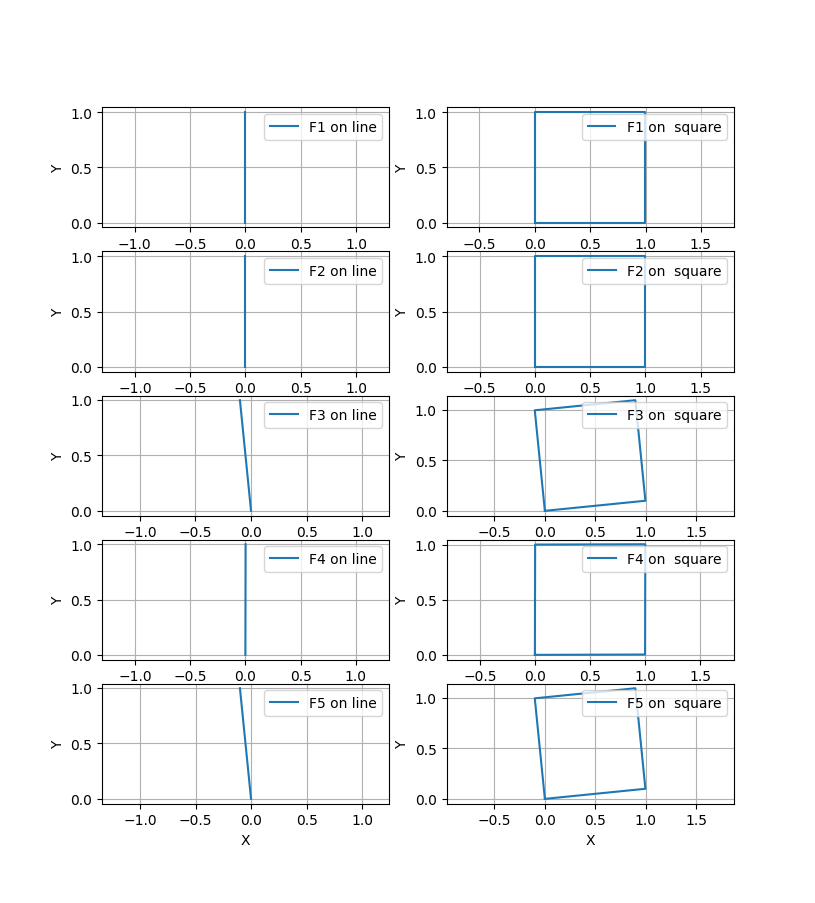
\includegraphics[scale=0.6]{HW2Q3_1.png}
        \caption{Deformation of Line and Square Element by Each $\vect{F}$}
    \end{figure}
It seems like there is a typo in the question statement. But the for the same conclusion.
I chose to use $\vect{F_5}$ and $\vect{F_2F_3}$ to show the $\vect{F_5}$ can be decomposed into a rigid 
body rotation $\vect{F_3}$ and a stretch of element $\vect{F_2}$. The result is shown in Figure 2.
    \begin{figure}[htbp]
        \center
        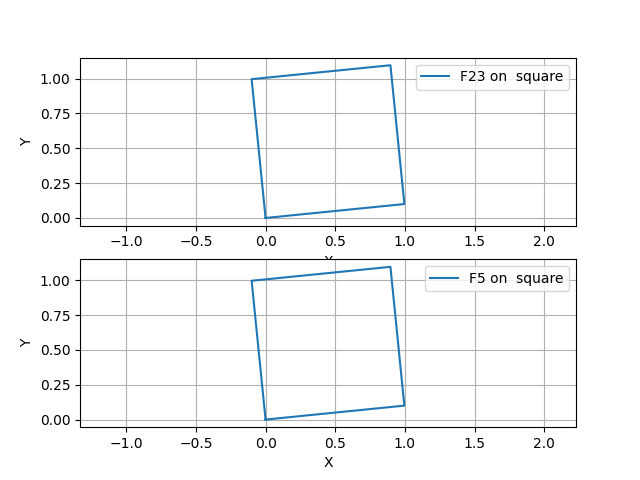
\includegraphics[scale=0.6]{HW2Q3_2.png}
        \caption{Deformation of the Square Element by $\vect{F_5}$ and $\vect{F_2F_3}$}
    \end{figure}

\newpage
\section*{Q4}
\begin{align*}
dl_{f1,F4} &= 0.002\\
dl_{f2,F4} &= 0.001\\
% dl_{f1,F5} &= 0.0009999999999998899\\
% dl_{f2,F5} &= 0.0009999999999998899\\
d\theta_{f1f2,F4} &= -0.00499 rads  = 0.2807 degree\\
\end{align*}
\end{document}